\documentclass{article}
\usepackage{amsmath}
\usepackage{graphicx}
\usepackage{lipsum}  % For generating dummy text (remove in your actual document)
\usepackage[a4paper, margin=2.5cm]{geometry} % Specify A4 paper size and margins
\usepackage{draftwatermark}
% Define the watermark content, color, and position
\usepackage{xcolor}

\definecolor{lightgray}{rgb}{0.9,0.9,0.9}

\SetWatermarkText{MCT 461: Kalman filter analysis of a mechatronics system (S.C. Nwafor)}
\SetWatermarkScale{1}
\SetWatermarkColor{lightgray}
\SetWatermarkAngle{45}

\title{MCT 461: Kalman Filtering and Analysis of Nonlinear Mechatronics Systems}
\author{Nwafor, Solomon Chibuzo\footnote{Department of Mechatronic Engineering, University of Nigeria, Nsukka.\\ Email: solomon.nwafor@unn.edu.ng}}
\date{October 09, 2023}

\begin{document}

\maketitle

\section{Introduction}
Mechatronic systems are complex systems that integrate mechanical, electrical, and electronic components. They are often nonlinear, meaning that their behavior cannot be accurately described by linear equations. This nonlinearity can make it difficult to design and control mechatronic systems.\\
\indent An example of a simple nonlinear mechatronics system is a pendulum as shwon in Figure~\ref{fig1}. A pendulum is a mass suspended from a pivot point by a massless rod. The pendulum can swing back and forth under the influence of gravity. The dynamics of a pendulum are nonlinear because the gravitational force acting on the pendulum depends on the pendulum's angle. When the pendulum is at its vertical equilibrium position, the gravitational force is directly downward. However, when the pendulum is displaced from its equilibrium position, the gravitational force has a horizontal component as well. This horizontal component of the gravitational force is what causes the pendulum to swing back and forth.\\
\indent The Kalman filter is a widely used estimation technique in many fields, including the nonlinear mechatronics systems. It uses a \emph{recursive algorithm} that relies on a state space model to estimate the state of a system, based on a set of noisy measurements. By combining the model predictions with the measurement, the filter provides an accurate and optimal estimate of the system state. In the case of nonlinear mechatronic systems, the Kalman filter can be used to estimate the states of mechanical and electrical components in real-time. Moreover, it is also useful in detecting and diagnosing faults, which is crucial in maintaining mechatronic systems.
\\
\begin{figure}[h!]
\begin{center}
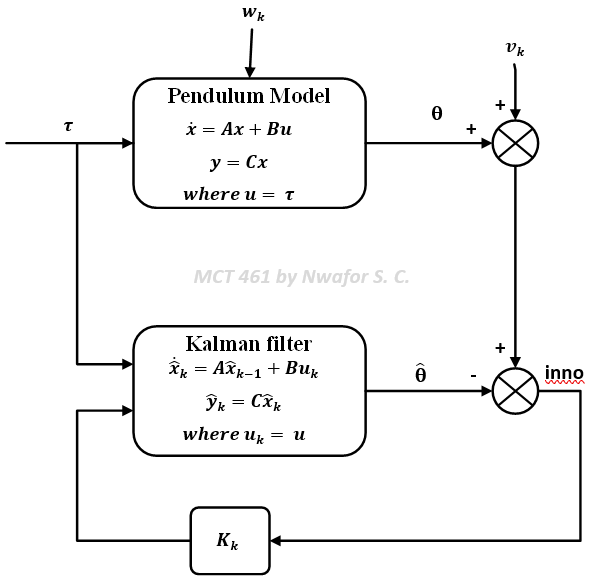
\includegraphics[width=10.0cm]{Kalman_filter_model_pendulum}
\caption{State Estimation of a PendulumModel}
\label{fig1}
\end{center}
\end{figure}
\\
The Kalman filter combines the measurement $\theta$, and the prediction $\hat{\theta}$ to find the optimal estimate of the pendulum position. From the pendulum model, we have:\\

\begin{align}
&\dot{x}_{k} = A x_{k} + B u_{k} + w_{k} \label{eq2}\\
&y_{k} = C x_{k} + v_{k} \label{eq1}
\end{align}
\\
where $x_{k} = \begin{bmatrix}

\theta \\ \dot{\theta}
\end{bmatrix} $
\\
$w_{k} = Process noise:$ This is derived from Gaussian distribution with zero mean and covariance that is $w_{k} \sim N(0, Q)$ as shown in Figure~\ref{fig2}.
\\
\begin{figure}[h!]
\begin{center}
\includegraphics[width=6.0cm]{Process_noise}
\caption{Process Noise Distribution}
\label{fig2}
\end{center}
\end{figure}
\\
$v_{k} = Measurement noise:$ This is derived from Gaussian distribution with zero mean and covariance that is $v_{k} \sim N(0, R)$ as shown in Figure~\ref{fig3}.
\\
\begin{figure}[h!]
\begin{center}
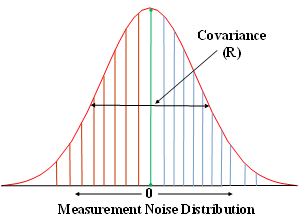
\includegraphics[width=6.0cm]{Measure_noise}
\caption{Measurement Noise Distribution}
\label{fig3}
\end{center}
\end{figure}
\\
Probability density function plays a crucial role in discussing the accuracy of Kalman filter as we can see in Figure~\ref{fig4}.
\\
\begin{figure}[h!]
\begin{center}
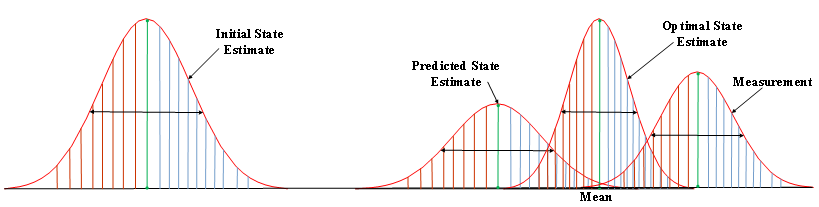
\includegraphics[width=15.0cm]{Estimate_predict}
\caption{Probability Density function of Kalman filter}
\label{fig4}
\end{center}
\end{figure}
\\
\section{Pendulum State Space Model}
Figure~\ref{fig5} shows a pendulum attached to a fixed body that swings freely with angular displacement. We can derive its governing differential equation and represent it in state space. We then apply Kalman filter to estimate the state (angular position) of the pendulum.\\

\begin{figure}[h!]
\begin{center}
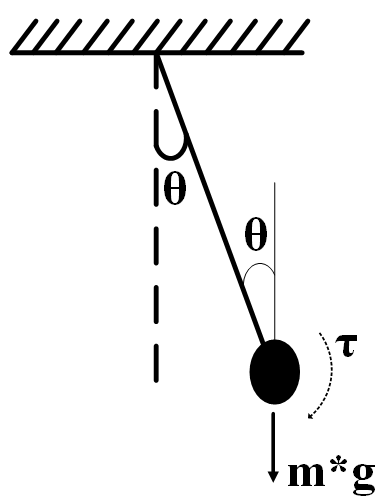
\includegraphics[width=3.5cm]{Simple_pendulum}
\caption{Pendulum Model}
\label{fig5}
\end{center}
\end{figure}
According to Newton's second law;
\begin{center}
\textit{Total torque = Moment of Inertia x Angular acceleration}
\end{center}
Also,
\begin{center}
\textit{Total torque = Pendulum torque + External torque}
\end{center}
\emph{Pendulum tirque = Force x Lever arm}
where Force = $-mg \sin\theta$ and Lever arm = $l$.
$$=-mg \sin\theta x l$$\\
External torque = $\tau$, Moment of inertia = $m.l^{2}$, and Angular acceleration = $\ddot{\theta} $\\
Therefore, $\tau - mg \sin\theta x l$ = $m.l^{2} x \ddot{\theta}$\\
Making the highest differential, we have:
\begin{equation}
\label{eg6}
\ddot{\theta} = \dfrac{\tau}{m.l^{2}} - \dfrac{g \sin\theta}{l}
\end{equation}
Equation (\ref{eg6}) is a nonlinear equation. For small angle of $\theta$, we use the approximation $\sin\theta\simeq\theta$ in (\ref{eg6}).
Therefore,\\
\begin{equation}
\label{eg7}
\ddot{\theta} = - \dfrac{g \theta}{l} + \dfrac{\tau}{m.l^{2}}
\end{equation}
\textbf{Reformulating \ref{eg7} into state space:}\\
TThe state space of a dynamical system, such as a pendulum, refers to the set of all possible system states. A system state is a complete description of the system's condition at a given time. However, transforming the pendulum equation into state space form results in:\\
\begin{flalign*}
&x_{1} = \theta ...... Angular.Pos (rad)\\
&x_{2} = \dot{x}_{1}....Angular.Vel (rad/s)\\
&\dot{x_{2}} = - \dfrac{g \theta}{l} + \dfrac{\tau}{m.l^{2}}
\end{flalign*}
The state space representation in vector matrix form becomes;
\begin{align}
\begin{bmatrix}
\dot{x_{1}} \\ \dot{x_{2}}
\end{bmatrix} = \begin{bmatrix}
0 & 1 \\ - \dfrac{g \theta}{l} & 0
\end{bmatrix} \begin{bmatrix}
x_{1} \\ x_{2}
\end{bmatrix} + \begin{bmatrix}
0 \\ \dfrac{1}{m.l^{2}}
\end{bmatrix} \tau
\end{align}
\section{Pendulum State Estimation}

\textbf{\emph{What is the best way to estimate the pendulum position?}}\\
\indent It is by combining $\hat{x}^{-}_{k}$ (estimated pendulum position) and $\theta$ (actual measurement) to obtain the optimal estimate of the pendulum psotion. Kalman filter is a type of state observer designed for stochastic systems as seen in Figure~\ref{fig1}. Therefore, we have;\\
$$e = x_{k} - \hat{x}_{k-1} = \theta - \hat{\theta}$$ \\
$$\dot{e} = \dot{x}_{k} - \dot{\hat{x}}_{k} = A(e) - K_{k}(e)$$\\
In order to estimate the current state of the pendulum based on the initial state estimate, we have that;\\
$$\hat{x}_{k} = A \hat{x}_{k-1} + Bu_{k} + K_{k}(y_{k} - \hat{y}_{k})$$\\
where $\hat{x}_{k-1}$ is the initial estimated state, $K_{k}$ is the Kalman gain, $y_{k}$ is the actual position measurement$(\theta)$, and $\hat{y}_{k}$ is the Kalman measurement$(\hat{\theta})$.\\
From state space point of view, the output state is represented as:\\
$$\hat{y}_{k} = C \hat{x}^{-}_{k}$$\\
where $\hat{x}^{-}_{k} = A \hat{x}_{k-1} + Bu_{k}$. $\hat{x}^{-}_{k}$ predicts the current state $\hat{x}_{k}$ by using state estimate from the previous sample time step and current input. It is called \emph{Priori estimate}.\\
Therefore, we can rewrite \ref{eq1} as;
$$\hat{x}_{k} = \hat{x}^{-}_{k} + K_{k}(y_{k} - C \hat{x}^{-}_{k})$$ \\
The equation above has two parts: the first part, $\hat{x}^{-}_{k}$ is the prediction while the second part uses measurement, $y_{k}$ and  it with the prediction to \emph{update} the Priori estimate. This second part is known as \emph{update stage} and is also called \emph{Posteriori estimate}. In order words, kalman filter is a \emph{Two (2)} step processes.\\

\subsubsection{Prediction Step:}
\begin{equation}
\label{eq3}
\hat{x}^{-}_{k} = A \hat{x}_{k-1} + Bu_{k}
\end{equation}

\begin{equation}
\label{eq4}
\hat{P}^{-}_{k} = A \hat{P}_{k-1} A^{T} + Q
\end{equation}\\
The system model in in this step is used to calculate a Priori state estimate and the error covariance, $(\hat{P}^{-}_{k})$ of the Pendulum model. Where $\hat{P}^{-}_{k}$ is the measure uncertainty in the estimated state. This variance comes from the process noise and propagation of uncertainty. Note that $\hat{P}_{k-1}$ comes from the initial state estimate.\\

\subsubsection{Update Step:}
\begin{equation}
\label{eq5}
K_{k} = \dfrac{\hat{P}^{-}_{k} C^{T}}{C \hat{P}^{-}_{k} C^{T} + R}
\end{equation}

\begin{equation}
\label{eq6}
\hat{x}_{k} = \hat{x}^{-}_{k} + K_{k}(y_{k} - C \hat{x}^{-}_{k})
\end{equation}

\begin{equation}
\label{7}
\hat{P}_{k} = (I + K_{k} C) \hat{P}^{-}_{k}
\end{equation}\\

\indent The update uses the priori estimate calculated in the prediction step andupdates them to find their posteriori estimates of the states and error covariance. The Kalman gain is calculated such that it minimizes the posteriori error covariance, $\hat{P}_{k}$.

\section{Conclusion}

The Kalman filter is a valuable tool in the estimation of nonlinear mechatronic systems. These systems, which combine mechanical, electrical, and electronic components, often exhibit complex, nonlinear behaviors that cannot be accurately described by linear equations. In such scenarios, the Kalman filter utilizes a recursive algorithm and a state space model to estimate the system's state, even when dealing with noisy measurements. By effectively combining model predictions with measurements, the Kalman filter provides accurate and optimal estimates of the system's state. In the context of nonlinear mechatronic systems, it serves as a critical tool for real-time estimation of the states of various components, including mechanical and electrical elements. Furthermore, the Kalman filter also proves invaluable for fault detection and diagnosis, which is essential for the maintenance and proper functioning of mechatronic systems.

\section{Assessments}
1. How can the Kalman filtering estimation approach be utilized to determine the optimal angular position of a non-linear mechatronic system, specifically the simple pendulum shown in Figure~\ref{fig5}, modeled in SIMULINK? Please analyze the application of Kalman filtering in this system. Take acceleration due to gravity = $9.81\frac{m}{s^{2}}$, length of the pendulum as 2.5 m, mass of the pendulum = 2 kg, External applied torque = 0, sample time = 0.01. Initial angular position is pi/18 rad and initial angular velocity is $0\frac{rad}{s^{2}}$ Process noise, and measurement noise covariances are $10^{-4}$, and  $10^{-4}$ respectively.\\

2. How can Kalman filtering be used to estimate the optimal displacement of a non-linear mechatronic system, specifically the mass spring damper system shown in Figure~\ref{fig6}, where a chart with mass m = $3.2 kg$ is attached at one end by a damper and a spring fixed to the wall? Please model the physical system in SIMULINK and analyze the application of Kalman filtering. Take sample time to be 0.1 seconds, 1 m initial position and 0 m/s initial velocity. Process noise, and measurement noise covariances are $10^{-5}$, and  $10^{-4}$ respectively.

\begin{figure}[h!]
\begin{center}
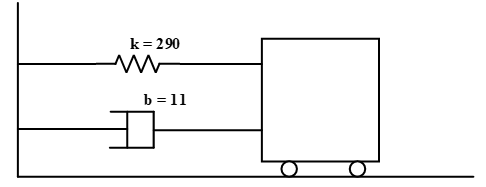
\includegraphics[width=10.0cm]{damp_spring}
\caption{Mass Sping Damper System on a Track}
\label{fig6}
\end{center}
\end{figure}

\section{References}

1. Design and use Kalman filters in MATLAB and Simulink: https://bit.ly/3i4VKwG\\
2. An Introduction to the Kalman Filter by G. Bishop (2001) https://courses.cs.washington.edu/courses/cse571/03wi/notes/welch-bishop-tutorial.pdf 
\end{document}
